\section{GroupTesting}
\begin{frame}\frametitle{Group Testing}
	\begin{figure}[t]
		\centering
		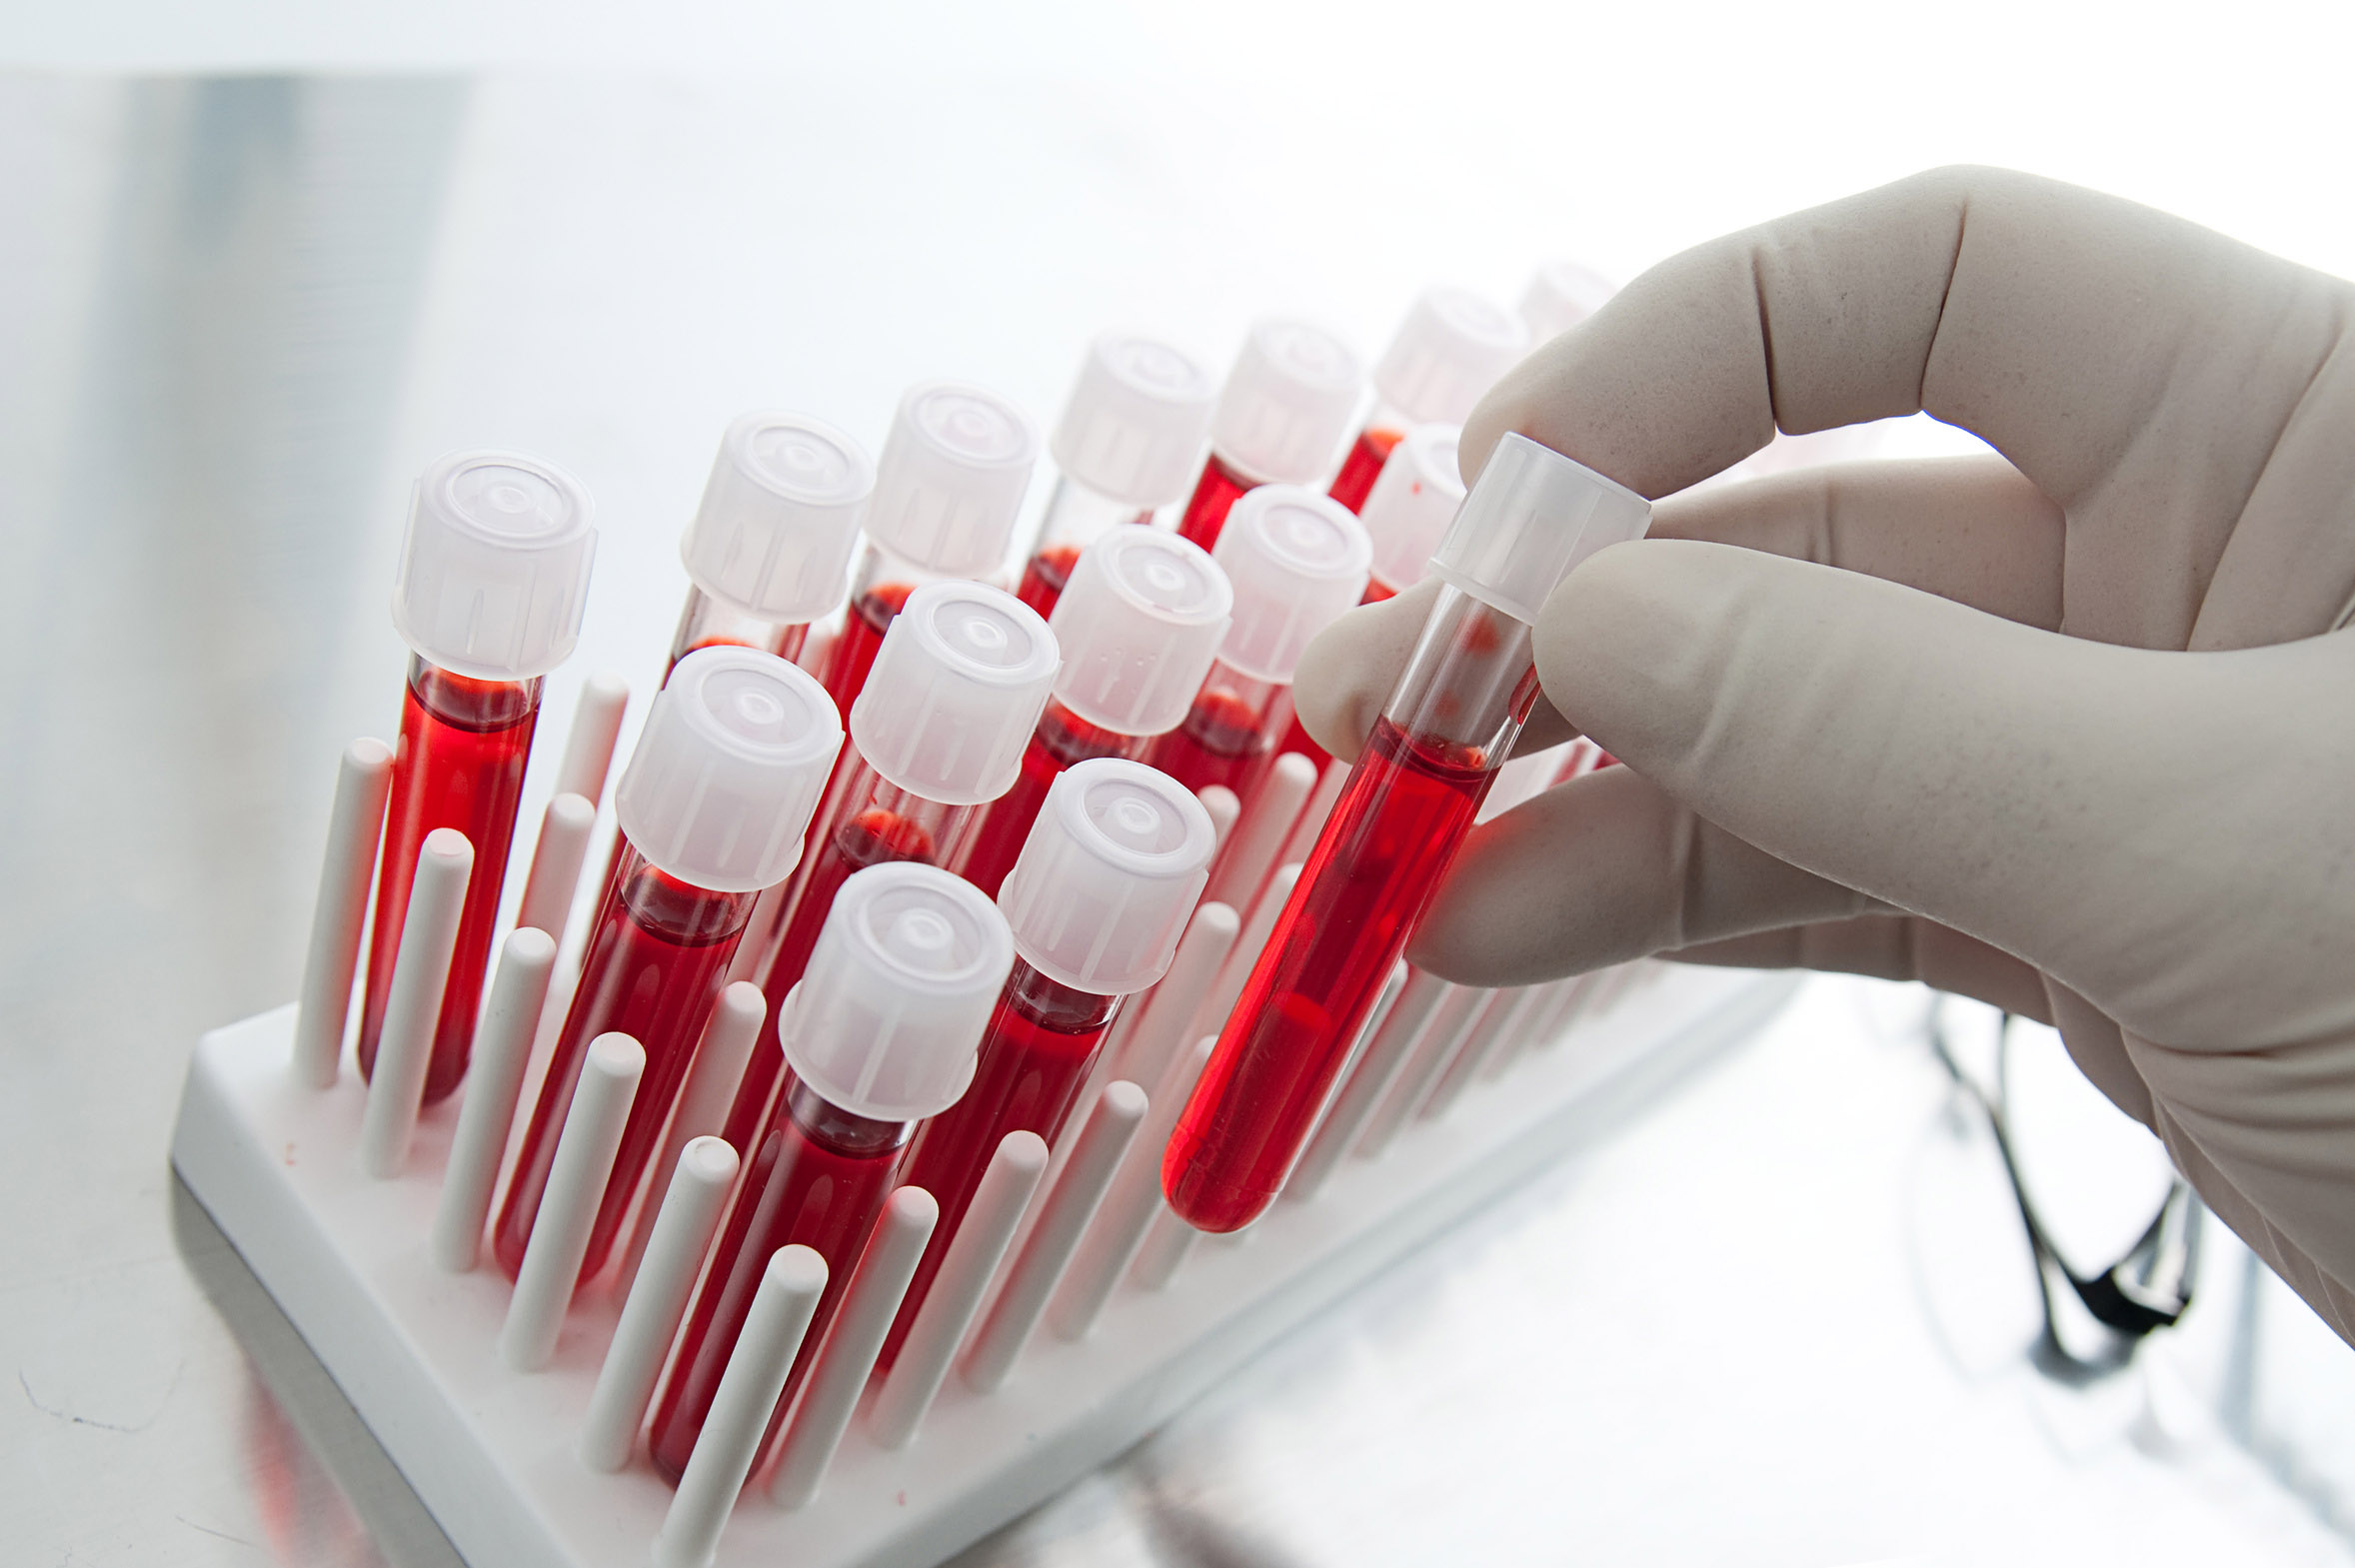
\includegraphics[width=1.8in]{\gt_figpath/grouptest_testubes.jpg}
	\end{figure}

\begin{itemize}
	\item II World War - detect all soldiers with syphilis
	\item Tests performed on efficiently pooled groups of items
	\item Least no. of tests ($m$) to identify $K$ defective items from $N$ items
\end{itemize}	

\end{frame}

%%%-------------------------------------------------------------------------------------------
\begin{frame}\frametitle{Group Testing}
\alert{Example}
\vspace{-0.3in}
	\begin{figure}[t]
		\centering
		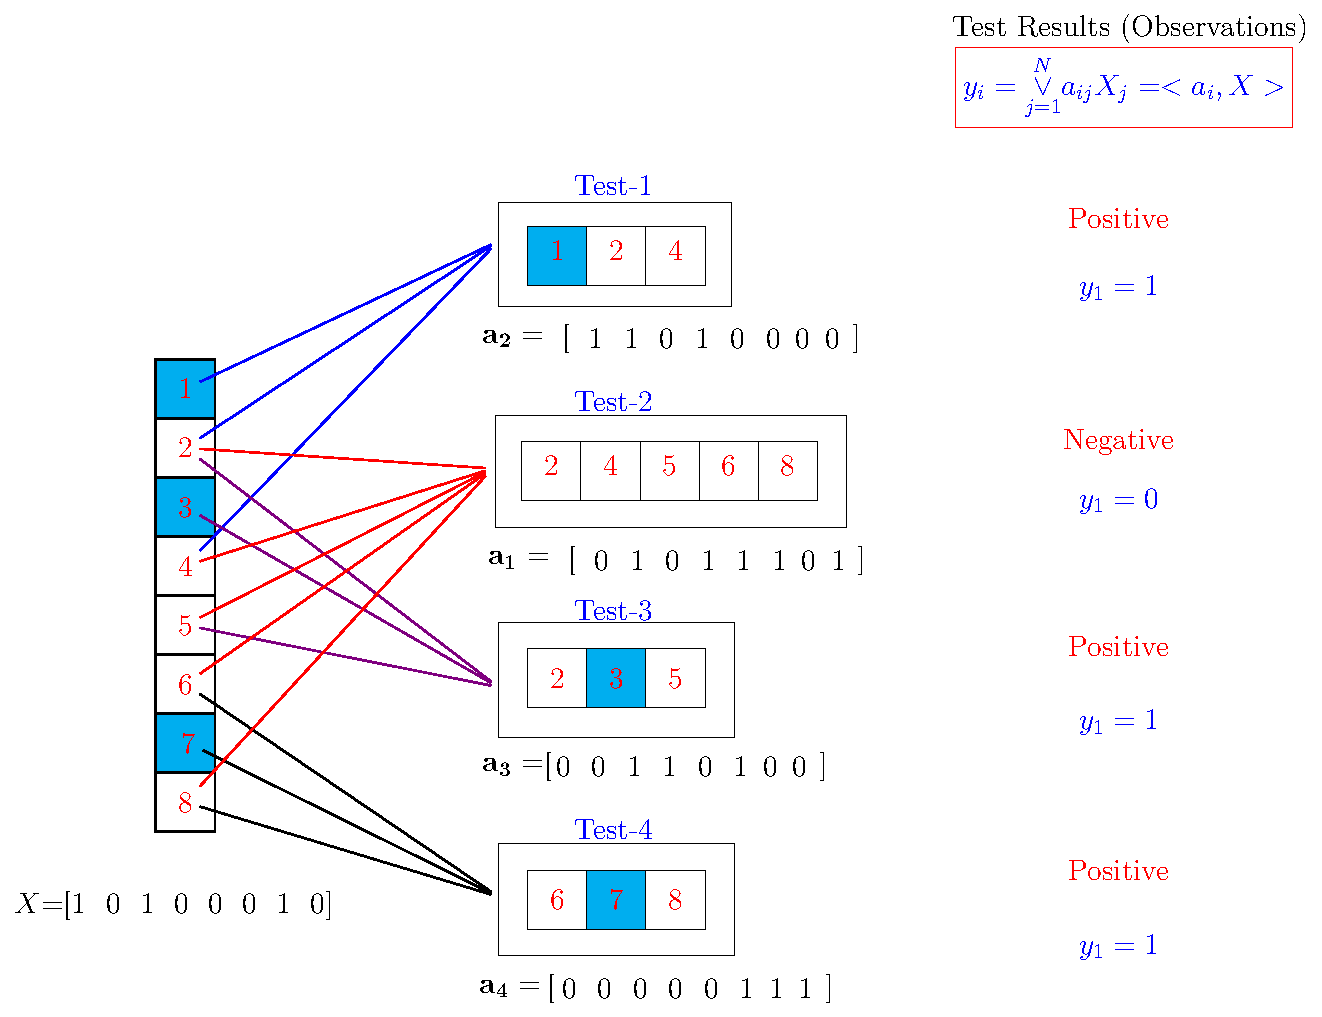
\includegraphics[width=4.2in]{\gt_figpath/grouptesting_example.pdf}
	\end{figure}
\end{frame}


%%----------------------------------------------------------------------------------
\begin{frame} \frametitle{Group Testing}
\begin{figure}[t]
\centering
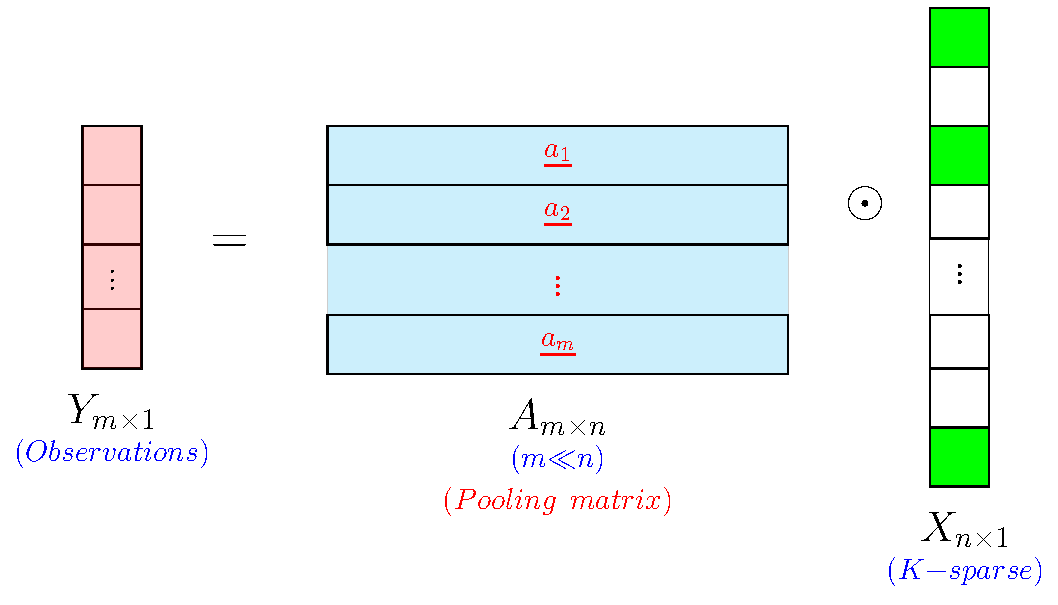
\includegraphics[width=3.4in]{\gt_figpath/A_times_X_group_testing.pdf}
\end{figure}

\begin{block}
	{
		\[ \small \underset{\color{blue}(Observation \ vector)}{Y_{m \times 1}} = A \odot X = \begin{bmatrix}
		{<a_1,X>} \\
		{<a_2,X>}  \\
		\vdots  \\
		{<a_m,X>}
		\end{bmatrix} \ \   <a_i , X> = \overset{N}{\underset{j=1 }{\vee}} a_{ij}X_j  \] }
		
\end{block}
\end{frame}

%%%------------------------------------------------------------------------------
\begin{frame}{Group Testing}
\begin{block}{Differences}
\begin{itemize}
\item Differs from CS: OR operation, non-linear
\item So the previous bin detection matrix would not work
\end{itemize}
\end{block}	

\onslide<2->			
\begin{block}{Singleton detection}			
{
 \tiny
$$
			\begin{bmatrix}
		H_1 \\
		\overline{H_1}
\end{bmatrix}
=
\begin{bmatrix}
					\bf{b_1} & \bf{b_2} & \bf{b_3} & \cdots & \bf{b_{n-1}}\\
				   	\bf{\overline{b_1}} & \bf{\overline{b_2}} & \bf{\overline{b_3}} & \cdots & \bf{\overline{b_{n-1}}} \end{bmatrix}
=
 \begin{bmatrix}
		0      & 0   & 0 & \cdots & 1 &  1 \\
		0      & 0   & 0 & \cdots & 1 &  1  \\
		\vdots & \vdots & \vdots & \ddots & \vdots & \vdots \\
		0      & 0   & 1 & \cdots & 1 &  1  \\
		0      & 1   & 0 & \cdots & 0 &  1  \\
		-- & -- & -- & -- & -- & --  \\
        1      & 1   & 1 & \cdots & 0 &  0 \\
		1      & 1   & 1 & \cdots & 0 &  0  \\
		\vdots & \vdots & \vdots & \ddots & \vdots & \vdots \\
		1      & 1   & 0 & \cdots & 0 &  0  \\
		1      & 0   & 1 & \cdots & 1 &  0  \\
\end{bmatrix}
$$
}
\alert{Note:} If a checknode is a singleton, with $i$th bit-node participating, then the observation vector is the $i$th column of $A$.

\begin{itemize}
\item Singleton - if the {\color{blue}weight of first two observation} vectors together is{ \ \color{blue} $L$}.
\item {\color{blue}Position} of the defective item is - {\color{blue} decimal value of the 1st observation vector}.
\end{itemize}    				
\end{block}					
\end{frame}

%%%---------------------------------------------------------------------------------
\begin{frame}\frametitle{Group Testing}
\vspace*{-0.1in}
  \begin{block}{Measurement matrix ($A_{m\times n}$)}
  {\centering
  $A_{m \times n}  = \underset{\color{blue} (d-left \ regular \ Graph)}{\bf G_{\frac{m}{6} \times n}} {\Large \bf \color{red} \otimes} \underset{\color{blue} (Singleton \ identifier)}{\bf H_{6 \times n}}$ \\
  \vspace{6pt}
  Let, $\bf{b_i}$ denote the {\color{blue}$L$-bits binary representation of the integer $i-1$}, $L=\lceil \log_2{n} \rceil$.
   {\small \[ H = \begin{bmatrix}
					\bf{b_1} & \bf{b_2} & \bf{b_3} & \cdots & \bf{b_{n-1}}\\
				   	\bf{\overline{b_1}} & \bf{\overline{b_2}} & \bf{\overline{b_3}} & \cdots & \bf{\overline{b_{n-1}}}\\
					\bf{b_{i_1}} & \bf{b_{i_2}} & \bf{b_{i_3}} & \cdots & \bf{b_{i_{n-1}}}\\
				   	\bf{\overline{b_{i_1}}} & \bf{\overline{b_{i_2}}} & \bf{\overline{b_{i_3}}} & \cdots & \bf{\overline{b_{i_{n-1}}}}\\
				   	
					\bf{b_{j_1}} & \bf{b_{j_2}} & \bf{b_{j_3}} & \cdots & \bf{b_{j_{n-1}}}\\
				   	\bf{\overline{b_{j_1}}} & \bf{\overline{b_{j_2}}} & \bf{\overline{b_{j_3}}} & \cdots & \bf{\overline{b_{j_{n-1}}}} \end{bmatrix} \]
$s_1=(i_1, i_2, \cdots, i_{n-1})$ and $s_2=(j_1, j_2, \cdots, j_{n-1})$ are permutations }}
 \end{block}

\begin{block}{Decoding procedure}
\begin{itemize}
\item  Identify and decodes singletons using weights of the observation vector
\item Identify and resolve doubletons by guessing to satisfy the first pair of observation vectors and checking if the guess satisfies the other two pairs of observations
\item The iteration continues until no doubletons can be resolved
\end{itemize}

\end{block}
\end{frame}

%----------------------------------------------------------------------------------------------------------------------------------
\begin{frame} \frametitle{Main results for group testing}
\begin{block}{Non-adaptive Group Testing (Noiseless and Noisy)}
\begin{itemize}
\item Recovers $(1-\epsilon)K$ items w.h.p.
\item Samples: $m = \Theta(K \log_2 \frac{N}{K})$ is order optimal
\item Computational complexity: $O(K \log \frac{N}{K})$  (order optimal)
\end{itemize}
\end{block}

\end{frame}

%----------------------------------------------------------------------------------------------------------------------------------
\begin{frame}{Conclusion}
\begin{itemize}
  \item Review of a simple message passing decoder called the peeling decoder
  \item Density evolution as a tool to analyze its asymptotic performance
  \item Applications 
    \begin{itemize}
      \item Sparse Fourier transform computation
      \item Compressed sensing type sparse recovery problems
    \end{itemize}
\end{itemize}
\end{frame}
	
%--------------------------------------------------------------------
\begin{frame}\frametitle{Questions?}
	\begin{figure}[t]
		\centering
		
\includegraphics[width=2.8in]{\gt_figpath/questions}
	\end{figure}
	\centering
	\color{blue}
	\Huge{Thank you!}
\end{frame}
